% ============================================================
% FINAL PROJECT REPORT - ENGLISH VERSION
% Project 14: Structured Document-Level Translation (doctrans)
% Course: CSC15012 - Applications of NLP in Industry
% Student: Le Dinh Minh Quan - 23127460 - 23CNTThuc
% ============================================================
\documentclass[12pt,a4paper]{article}

\usepackage[utf8]{inputenc}
\usepackage{geometry}
\geometry{left=2.3cm, right=2.3cm, top=2.5cm, bottom=2.5cm}
\usepackage{setspace}
\setstretch{1.25}
\usepackage{graphicx}
\usepackage{float}
\usepackage{booktabs}
\usepackage{longtable}
\usepackage{tabularx}
\usepackage{array}
\usepackage{hyperref}
\hypersetup{colorlinks=true, linkcolor=blue, urlcolor=blue, citecolor=blue, breaklinks=true}
\usepackage{xurl}
\usepackage{seqsplit}
\usepackage{listings}
\usepackage{xcolor}
\usepackage{amsmath}
\usepackage{caption}
\usepackage{subcaption}
\usepackage{enumitem}
\usepackage{fancyhdr}
\usepackage{tikz}
\usetikzlibrary{shapes.geometric, arrows.meta, positioning, fit, backgrounds, shadows}

% --- Make long inline code / paths break gracefully ---
\sloppy
\tolerance=2000
\emergencystretch=3em
\hbadness=10000
\setlength{\parskip}{0.15em}

% Helper for breakable monospaced paths
\newcommand{\bpath}[1]{\seqsplit{#1}}
\newcommand{\btt}[1]{\texttt{\seqsplit{#1}}}

% New column type for tabularx: left-aligned and ragged-right with breaking
\newcolumntype{L}{>{\raggedright\arraybackslash}X}

\lstset{
  basicstyle=\ttfamily\small,
  breaklines=true,
  frame=single,
  backgroundcolor=\color{gray!10},
  keywordstyle=\color{blue},
  commentstyle=\color{green!60!black},
  stringstyle=\color{red!70!black},
  showstringspaces=false,
  tabsize=2
}

\pagestyle{fancy}
\fancyhf{}
\fancyhead[L]{\small CSC15012 -- Final Project Report}
\fancyhead[R]{\small Le Dinh Minh Quan -- 23127460}
\fancyfoot[C]{\thepage}

% ============================================================
\begin{document}

% --- TITLE PAGE ---
\begin{titlepage}
\centering
\vspace*{0.5cm}

% HCMUS LOGO: upload logo_hcmus.png to Overleaf and uncomment the next line
\IfFileExists{logo_hcmus.png}{\includegraphics[width=3.5cm]{logo_hcmus.png}\\[0.5cm]}{}

{\large \textbf{VIETNAM NATIONAL UNIVERSITY HO CHI MINH CITY}}\\[0.3cm]
{\Large \textbf{UNIVERSITY OF SCIENCE}}\\[0.3cm]
{\large Faculty of Information Technology}\\[1.5cm]

{\LARGE \textbf{FINAL PROJECT REPORT}}\\[0.5cm]
{\large Course: \textbf{CSC15012 -- Applications of Natural Language\\ Processing in Industry}}\\[1.5cm]

{\Large \textbf{Project 14:}}\\[0.3cm]
{\Large \textbf{Structured Document-Level Translation}}\\[0.3cm]
{\large Structure-Preserving, Context-Aware Machine Translation (\texttt{doctrans})}\\[2cm]

\begin{tabular}{ll}
\textbf{Student:} & Le Dinh Minh Quan \\
\textbf{Student ID:} & 23127460 \\
\textbf{Class:} & 23CNTThuc \\
\end{tabular}

\vfill
{\large Ho Chi Minh City, 2026}
\end{titlepage}

\tableofcontents
\newpage

% ============================================================
\section{Introduction}
% ============================================================

Real-world translation rarely operates on bare sentences. It operates on \textbf{structured documents}: Markdown READMEs, HTML help pages, JSON localization bundles, and product docs. Each such document carries two things a localizer must respect at once -- the \textbf{prose}, which must change language, and the \textbf{structure} (headings, lists, tables, fenced code, links, inline markup, and runtime placeholders such as \texttt{\{name\}}, \texttt{\%s}, \texttt{\$\{VAR\}}) which must survive \textit{byte-stably}.

Feeding such a document straight into a raw machine-translation (MT) model corrupts it: the model rewrites code blocks, translates URL targets and placeholders, drops table pipes, mangles heading hashes, and reflows lists. The output may read fluently yet be \textbf{structurally broken} -- a page that fails to render, an i18n file that breaks string interpolation at runtime, or a code sample that no longer compiles.

This project implements \textbf{\texttt{doctrans}}, a complete \textbf{Structured Document-Level Translation} system built around a single principle: \emph{the model never sees structure, and the structure layer never sees the model}. A deterministic localization spine parses each format, extracts only translatable leaf prose, masks every non-translatable span behind opaque sentinels, translates that prose with \emph{document-level context}, restores the masks, and reassembles the document in place so it reproduces byte-for-byte except for the translated text. The system delivers:

\begin{itemize}
  \item A deterministic \textbf{structure layer} (parse $\rightarrow$ mask $\rightarrow$ translate $\rightarrow$ restore $\rightarrow$ reassemble $\rightarrow$ validate) covering Markdown / HTML / JSON / plain text.
  \item A \textbf{trainable MT core} (the NLP heart) -- a fine-tuned \texttt{m2m100} sequence-to-sequence model using concatenation-based document context (concat-$k$).
  \item A \textbf{deterministic agent} with five explicit decision gates (D1--D5) that hard-gate placeholder-retention and structure-preservation.
  \item Production-ready \textbf{deployment}: FastAPI REST API, Gradio demo UI, CLI, Docker, and a one-button Colab H100 autopilot.
\end{itemize}

The default translation direction is \textbf{English $\rightarrow$ French} (configurable). The whole pipeline runs fully offline (line/regex parsers + dictionary MT + pure-python metrics) and upgrades to the fine-tuned \texttt{m2m100} core plus optional native parsers when the heavy dependencies are present.

\textbf{Project Resources (public):}
\begin{itemize}\setlength\itemsep{0.15em}
  \item \textbf{GitHub repository (source code):} \url{https://github.com/ledinhminhquan/14_Document_Level_Translation}
  \item \textbf{Trainable MT core (HF Hub):} \texttt{facebook/m2m100\_418M} (MIT, 1024 positions) -- fine-tuned via the included Colab H100 autopilot notebook.
  \item \textbf{Deployment surface:} FastAPI REST API + Gradio demo (\texttt{doctrans serve --ui}), Docker / \texttt{docker-compose}, and the Hugging Face Space-ready image (offline-degradable). The system is fully deployable but is \emph{not} currently hosted at a live public URL.
\end{itemize}

\textbf{Honesty note on results.} The numbers reported here are the \textbf{verified offline / synthetic-spine figures} produced by \texttt{doctrans evaluate} on the offline seed (small Markdown docs + gold French + an en$\rightarrow$fr dictionary). They establish the floors and the structure-preservation guarantees; the full fine-tuned MT numbers come from the real Colab H100 training run. Every dataset id, model id, license, and configuration value is taken directly from the project's verified design documents.

% ============================================================
\section{Business Problem Definition}
% ============================================================

\subsection{Context and Motivation}

Localization is a recurring, high-volume cost for any organization that ships documentation, product UI, or content in more than one language. The pain is not only ``translate the words'' but ``translate the words \emph{without breaking the artifact}'':
\begin{itemize}
  \item \textbf{Structural corruption}: raw MT eats list markers, translates URLs and placeholders, and mangles tables/code -- producing output that fails to render or breaks at runtime.
  \item \textbf{Discourse drift}: sentence-by-sentence translation discards document context, so pronouns, formality, and terminology drift across a page.
  \item \textbf{Manual post-editing cost}: localization engineers spend disproportionate effort fixing structure and consistency, not language.
\end{itemize}

\subsection{Target Users and Stakeholders}

\begin{itemize}
  \item \textbf{Localization engineers}: translate a JSON/HTML bundle without breaking interpolation or markup.
  \item \textbf{Documentation writers}: ship a French README/docs page that still renders byte-stably.
  \item \textbf{Developers / i18n owners}: wire MT into a CI/CD localization step behind a REST API with a fail-soft contract.
  \item \textbf{MT researchers}: measure whether document context actually helps (the 2$\times$2 ablation).
\end{itemize}

\subsection{Problem Statement}

Given a structured document in a supported format, the system must:
\begin{enumerate}
  \item \textbf{Preserve structure byte-stably}: headings, lists, tables, code blocks, links, inline markup, and placeholders are reproduced exactly.
  \item \textbf{Translate the prose} with document-level context (concat-$k$) for discourse consistency.
  \item \textbf{Guarantee placeholder-retention}: every masked non-translatable span returns exactly once -- a hard, non-negotiable gate.
  \item \textbf{Fail soft}: structure-breaking or low-confidence output is flagged for human review and the source is kept, never presented as final.
\end{enumerate}

\subsection{Why NLP is Required}

The translatable prose carries context, pronouns, register, and terminology that demand a learned, context-aware sequence-to-sequence model. Rule-based or dictionary substitution is acceptable only as an offline floor; it cannot produce fluent, agreement-correct French or maintain discourse consistency across a document. The \textbf{only learned component} of the system is the MT core; everything else is deterministic, testable code. This is precisely where the machine learning -- and the evaluation -- lives.

\subsection{Success Metrics}

\begin{table}[H]
\centering
\caption{System success metrics}
\begin{tabular}{lll}
\toprule
\textbf{Type} & \textbf{Metric} & \textbf{Target} \\
\midrule
Business & Localization post-edit (needs-review) rate & Reduce vs.\ manual \\
Business & Structurally-broken output rate & $\approx$ 0\% (hard gates) \\
Technical & chrF (headline MT quality) & Beat all baselines \\
Technical & Placeholder-Retention Rate (PHR) & $=1.0$ (hard) \\
Technical & Structure-Preservation Score (SPS) & $=1.0$ target \\
\bottomrule
\end{tabular}
\end{table}

% ============================================================
\section{Development Infrastructure \& Tooling}
% ============================================================

\subsection{Repository Structure}

The project follows a production-ready Python package structure, mirroring the public GitHub repository \url{https://github.com/ledinhminhquan/14_Document_Level_Translation} one-to-one. The Python package \texttt{doctrans} is organized by responsibility: the deterministic \textbf{structure layer} (\texttt{docparse/}), the \textbf{trainable MT core} (\texttt{mt/}, \texttt{training/}), the \textbf{deterministic agent FSM} (\texttt{agent/}), serving (\texttt{api/}), and the operational tooling (\texttt{autoreport/}, \texttt{monitoring/}, \texttt{automation/}, \texttt{grading/}). The MT plumbing (translator, training loop, pure-python metrics) is reused directly from the sibling P13 \texttt{s2st} project. There are \textbf{15 rubric-aligned docs} under \texttt{docs/}.

\begin{lstlisting}[basicstyle=\ttfamily\footnotesize]
14_Document_Level_Translation/
|-- src/doctrans/                  # Python package
|   |-- config.py, cli.py          # DocTransConfig + single CLI entrypoint
|   |-- logging_utils.py           # logs to stderr; stdout stays pipeable JSON
|   |-- data/                      # opus-100 / news_commentary loaders,
|   |   |                          #   download (streaming probes), and
|   |   +-- samples.py             #   offline seed (md docs + en->fr dict)
|   |-- models/                    # model registry
|   |-- docparse/                  # THE STRUCTURE LAYER
|   |   |-- segment.py, mask.py    #   Segment + [[PHn]] sentinel masking
|   |   |-- markdown_doc.py        #   markdown-it (native) parser
|   |   |-- html_doc.py            #   beautifulsoup4 / stdlib parser
|   |   |-- json_doc.py            #   stdlib json walker
|   |   |-- plain_doc.py           #   regex/line fallback (the floor)
|   |   |-- router.py              #   format detect + degradation ladder
|   |   +-- structure_score.py     #   SPS = struct x markup x PHR
|   |-- mt/                        # THE TRAINABLE MT CORE (reused from P13)
|   |   |-- translator.py          #   m2m100 + DictionaryTranslator
|   |   +-- context.py             #   concat-k context assembly (<BRK>)
|   |-- training/                  # train_mt, train_baseline, evaluate,
|   |   |                          #   tune, metrics (chrF / BLEU, pure-python)
|   |-- agent/                     # THE DETERMINISTIC AGENT
|   |   |-- state.py, policy.py    #   FSM state + D1-D5 gates
|   |   |-- tools.py               #   uniform tool contract + ToolTrace
|   |   |-- llm_orchestrator.py    #   optional Anthropic brain (OFF default)
|   |   +-- doctrans_agent.py      #   the FSM driver
|   |-- api/                       # FastAPI + Gradio
|   |   |-- main.py, app_combined.py  # /translate-text, /translate-document
|   |   |-- schemas.py, dependencies.py
|   |   +-- ui.py                  #   Gradio demo (mounted at /ui)
|   |-- analysis/                  # error_analysis + latency
|   |-- autoreport/                # artifact_loader, charts, report_pdf,
|   |   |                          #   slides_pptx (auto report + slides)
|   |-- monitoring/                # drift_report (operational monitor-log)
|   |-- automation/autopilot.py    # one-button full pipeline
|   +-- grading/checklist.py       # rubric completeness self-check
|-- configs/                       # YAML configs (DocTransConfig)
|-- docs/                          # 15 rubric-aligned docs (.md)
|-- data/  models/  sample_data/   # data scripts, ckpt placeholder, seed docs
|-- tests/                         # CPU-only, offline pytest
|-- notebooks/                     # DocTrans_Colab_Training_H100_AUTOPILOT.ipynb
|-- app/  deploy/  scripts/        # demo app, deploy helpers, scripts
|-- Dockerfile, docker-compose.yml # container deployment
|-- pyproject.toml, requirements*.txt
|-- Makefile, .github/workflows/ci.yml
+-- README.md, LICENSE (MIT)
\end{lstlisting}

\subsection{Technology Stack}

\begin{table}[H]
\centering
\caption{Technology stack}
\small
\begin{tabularx}{\linewidth}{@{} l L @{}}
\toprule
\textbf{Component} & \textbf{Technology} \\
\midrule
Language & Python 3.12 \\
Version Control & Git + GitHub (public repo) \\
ML Framework & PyTorch + HuggingFace Transformers (\texttt{Seq2SeqTrainer}), Datasets, Accelerate \\
Trainable MT core & \texttt{facebook/m2m100\_418M} ($\sim$418M params, MIT, 1024 positions) \\
Stronger alternatives & \texttt{facebook/mbart-large-50-many-to-many-mmt}, \texttt{facebook/nllb-200-distilled-600M} (CC-BY-NC, flag) \\
Lite alternative & \texttt{Helsinki-NLP/opus-mt-en-fr} (Apache-2.0, 75M, 512 positions) \\
Baselines & Zero-shot MT, DictionaryTranslator (offline), identity copy-source \\
Structure parsers & \texttt{markdown-it-py} + \texttt{mdformat}, \texttt{beautifulsoup4}, \texttt{python-docx}, stdlib \texttt{json} (all optional, degradation ladder) \\
Metrics & \texttt{sacrebleu} + \texttt{evaluate} (chrF/BLEU) with pure-python fallback \\
API & FastAPI + Uvicorn \\
UI & Gradio (mounted under FastAPI at \texttt{/ui}) \\
Containerization & Docker + Docker Compose; Hugging Face Space-ready image \\
Training GPU & Google Colab H100 80GB (auto-adapts A100 / L4 / T4) \\
\bottomrule
\end{tabularx}
\end{table}

\subsection{Training Workflow \& Autopilot Pipeline}
\label{subsec:workflow}

The end-to-end training-to-deployment workflow is automated both by the CLI (\texttt{doctrans autopilot}) and by the Colab notebook \texttt{DocTrans\_Colab\_Training\_H100\_AUTOPILOT}. The notebook is resume-safe (\texttt{get\_last\_checkpoint}), GPU-auto-profiled, and Colab-safe (never reinstalls torch). It runs in a single Run-All:

\begin{figure}[H]
\centering
\resizebox{\linewidth}{!}{%
\begin{tikzpicture}[
  node distance=0.32cm,
  step/.style={rectangle, draw=black!60, rounded corners=2pt, thick,
              text width=13.5cm, inner sep=5pt, minimum height=0.75cm,
              align=center, font=\footnotesize},
  setup/.style={step, fill=gray!15},
  train/.style={step, fill=orange!15},
  eval/.style={step, fill=blue!15},
  deploy/.style={step, fill=green!15},
  arrow/.style={-{Stealth[length=2mm]}, thick}
]

\node[setup] (s1) {\textbf{1. Setup (Colab)}: mount Drive, set \texttt{DOCTRANS\_*\_DIR} + \texttt{HF\_HOME}, GPU auto-profile (H100/A100/L4/T4), Colab-safe install};
\node[setup, below=of s1] (s2) {\textbf{2. Data}: streaming probes of \texttt{opus-100} (en-fr) + \texttt{news\_commentary} (en-fr); build concat-$k$ windows from per-article ids};
\node[train, below=of s2] (s3) {\textbf{3. Baseline}: dictionary MT + identity floor (instant, CPU) -- establishes the floor to beat};
\node[train, below=of s3] (s4) {\textbf{4. Train MT core}: \texttt{m2m100\_418M} fine-tune, \texttt{Seq2SeqTrainer}, concat-$k$ (k=2, \texttt{<BRK>}), bf16/tf32, resume-safe};
\node[eval, below=of s4] (s5) {\textbf{5. Evaluate}: chrF / BLEU / d-chrF + SPS (struct $\times$ markup $\times$ PHR); 2$\times$2 sentence-vs-context ablation};
\node[eval, below=of s5] (s6) {\textbf{6. Tune + analysis}: hyperparameter sweep; error analysis + latency benchmark (privacy-preserving, metadata-only)};
\node[deploy, below=of s6] (s7) {\textbf{7. Auto-gen report \& slides}: \texttt{report\_pdf} (PDF) + \texttt{slides\_pptx} (deck) from versioned JSON artifacts};
\node[deploy, below=of s7] (s8) {\textbf{8. Grade + bundle}: rubric self-check (\texttt{grading/checklist.py}) + submission zip};

\foreach \a/\b in {s1/s2, s2/s3, s3/s4, s4/s5, s5/s6, s6/s7, s7/s8}
  \draw[arrow] (\a) -- (\b);

\end{tikzpicture}%
}
\caption{The one-button autopilot workflow (\texttt{doctrans autopilot} / Colab notebook). Every step writes versioned JSON artifacts; the notebook is resume-safe so a restarted Colab session continues from the last checkpoint.}
\label{fig:workflow}
\end{figure}

\paragraph{Key workflow characteristics:}
\begin{itemize}\setlength\itemsep{0.15em}
  \item \textbf{Single-button Run-All}: data $\rightarrow$ baseline $\rightarrow$ train-mt $\rightarrow$ evaluate $\rightarrow$ tune $\rightarrow$ analysis $\rightarrow$ report.pdf + slides.pptx + grade + bundle.
  \item \textbf{Resume-safe}: \texttt{get\_last\_checkpoint(output\_dir)} $\rightarrow$ \texttt{trainer.train(resume\_from\_checkpoint=ckpt)}; survives Colab disconnects.
  \item \textbf{GPU auto-adapt}: \texttt{bf16 = torch.cuda.is\_bf16\_supported()}; on T4 falls back to \texttt{fp16=True, tf32=False}; \texttt{gradient\_checkpointing} when VRAM $<$ 40\,GB.
  \item \textbf{Streaming data probes}: \texttt{download\_dataset} uses \texttt{streaming=True} so opus-100 (1M) / news\_commentary (209K) never download huge files and hang.
  \item \textbf{Offline-degradable}: with no torch/network the same pipeline runs on the dictionary/identity baselines over the offline seed, so CI is green on CPU.
  \item \textbf{Versioned JSON}: every metric/run/model carries a \texttt{model\_version} and (for context models) \texttt{context:true}; outputs are diffable JSON, not free text.
\end{itemize}

% ============================================================
\section{Data Management}
% ============================================================

\subsection{Data Sources and Licenses}

A central, honestly-reported constraint of this project: \textbf{no Hugging Face corpus provides Markdown/HTML/JSON-structured parallel documents, and none provides clean en$\leftrightarrow$fr parallel data with explicit document-boundary metadata.} Therefore the MT core is fine-tuned on real sentence/paragraph parallel data, document-level context is reconstructed from corpora whose row order preserves intra-article adjacency, and \textbf{structure is 100\% synthetic} (real sentence pairs wrapped in Markdown/HTML/JSON). All ids and licenses below were verified live on the HF Hub.

\begin{table}[H]
\centering
\caption{Datasets and models with license flags (verified on the HF Hub)}
\small
\begin{tabularx}{\linewidth}{@{} l l l @{}}
\toprule
\textbf{Asset} & \textbf{Role} & \textbf{License / Flag} \\
\midrule
\texttt{Helsinki-NLP/opus-100} (\texttt{en-fr}) & MT fine-tune corpus (1M train) & \textbf{[FLAG: UNKNOWN]} \\
\texttt{Helsinki-NLP/news\_commentary} (\texttt{en-fr}) & document-context corpus (209.5K, real adjacency) & \textbf{[FLAG: UNKNOWN]} \\
\texttt{IWSLT/iwslt2017} (\texttt{en-fr}) & context alternative (talk order) & \textbf{[FLAG: CC-BY-NC-ND]} \\
\texttt{ParaCrawl/para\_crawl} (\texttt{enfr}) & permissive sentence corpus (no doc order) & CC0-1.0 (clean) \\
\texttt{facebook/m2m100\_418M} & MT core (default) & MIT (clean) \\
\texttt{facebook/nllb-200-distilled-600M} & stronger MT core (eval/research only) & \textbf{[FLAG: CC-BY-NC]} \\
Synthetic structured docs & structure train/eval (no HF corpus exists) & derived \\
Offline seed (md + gold fr + dict) & runs with no torch/network & local \\
\bottomrule
\end{tabularx}
\end{table}

\textbf{License hygiene.} The clean, redistributable path is \texttt{facebook/m2m100\_418M} (MIT) + the offline seed. Non-commercial assets (NLLB, IWSLT) are flagged and used only as research/eval baselines; the unknown-license corpora (opus-100, news\_commentary) are treated as research/educational. No flagged license is ever silently ``upgraded''.

\subsection{The Synthetic Structure Spine}

Two deterministic, seeded generators sit on top of the real sentence corpora:
\begin{enumerate}
  \item \textbf{Context-window builder}: groups consecutive same-article rows in \texttt{news\_commentary} (via the monotonic per-article \texttt{id}) into \texttt{(prev\_k \dots current)} windows for concat-$k$ training. Sentence-shuffled corpora (opus-100, ParaCrawl) cannot supply real context, so for those context is empty ($k=0$).
  \item \textbf{Structure wrapper}: programmatically wraps real sentence pairs in Markdown/HTML/JSON (headings, lists, tables, code blocks, links, placeholders) to train and evaluate structure preservation, plus a \textbf{seed of small gold structured docs} so tests, agent runs, and SPS/PHR/chrF evaluation all execute offline.
\end{enumerate}

\subsection{Document-Level Context (concat-$k$)}

Document context is realized as \textbf{concatenation-based context} (concat-$k$) -- the standard, architecture-free document-MT method. The $k$ previous source sentences are prepended to the current sentence, joined by a special \texttt{<BRK>} separator token, and the model is trained to output \textbf{only} the current target sentence (the \texttt{k-to-1} recipe). The default is \textbf{$k=2$, source-side}, with context \textbf{left-truncated} so the current sentence is never cut. This is why the model's position budget matters: \texttt{m2m100} (1024 positions) has comfortable headroom; \texttt{opus-mt} Marian (512) does not, limiting it to $k\approx1$--2.

\subsection{Preprocessing and Splits}

\begin{itemize}
  \item \textbf{Streaming probes}: datasets are probed with \texttt{streaming=True} to avoid multi-GB downloads.
  \item \textbf{Truncation strategy}: tokenize the current sentence first, reserve its tokens, then fill the remaining budget with previous sentences newest-first, dropping whole sentences (never partial) to preserve the \texttt{<BRK>} structure.
  \item \textbf{Splits}: opus-100 en-fr ships train 1.0M / validation 2.0K / test 2.0K; news\_commentary (209.5K, train only) is carved into a held-out context set with a fixed seed for reproducibility.
\end{itemize}

% ============================================================
\section{Model Selection \& Optimization}
% ============================================================

\subsection{The Trainable MT Core}

Only one component is trainable: the MT core. The structure layer and agent FSM are deterministic code. The default core is \textbf{\texttt{facebook/m2m100\_418M} (MIT)}, chosen for a permissive license (clean dependency path), a 1024-position budget that leaves headroom for prepended document context, and direct multilingual control (set \texttt{src\_lang}, force \texttt{forced\_bos\_token\_id} for the target). It reuses the P13 \texttt{s2st} seq2seq plumbing, so training and generation code are shared.

\begin{table}[H]
\centering
\caption{MT core options (the fallback ladder)}
\small
\begin{tabularx}{\linewidth}{@{} l l l L @{}}
\toprule
\textbf{Model} & \textbf{Params} & \textbf{License} & \textbf{When / notes} \\
\midrule
\texttt{m2m100\_418M} & $\sim$418M & MIT & \textbf{Default}; 1024 positions; ISO-639-1 codes \\
\texttt{mbart-large-50-mmt} & $\sim$611M & MIT (flag: not on repo) & 1024 positions; stronger than m2m100 \\
\texttt{opus-mt-en-fr} & $\sim$75M & Apache-2.0 & Lite, fastest; only 512 positions ($k\approx1$--2) \\
\texttt{nllb-200-distilled-600M} & $\sim$600M & CC-BY-NC (flag) & Research/eval baseline only \\
\texttt{madlad400-3b-mt} & $\sim$3B & Apache-2.0 & Zero-shot reference; LoRA/QLoRA only \\
\bottomrule
\end{tabularx}
\end{table}

\subsection{Baselines (the Floors to Beat)}

\begin{enumerate}
  \item \textbf{Identity (copy-source)}: copies the source as the ``translation'' -- the absolute floor.
  \item \textbf{Dictionary word-lookup}: an offline en$\rightarrow$fr dictionary (accent-stripped lookup), reused from P13's \texttt{DictionaryTranslator}; the no-torch/no-network floor.
  \item \textbf{Zero-shot MT}: the un-fine-tuned base checkpoint; the floor the fine-tuned system must clear (in both sentence-level and concat-$k$ variants).
\end{enumerate}

\subsection{Training Configuration}

\begin{table}[H]
\centering
\caption{\texttt{Seq2SeqTrainer} recipe (reused from P13)}
\begin{tabular}{ll}
\toprule
\textbf{Parameter} & \textbf{Value} \\
\midrule
Model & \texttt{facebook/m2m100\_418M} ($\sim$418M params) \\
Context & concat-$k$, $k=2$, source-side (\texttt{k-to-1}, \texttt{<BRK>}) \\
Max source length & 1024 (512 for Marian) \\
\texttt{predict\_with\_generate} & \texttt{True} (real chrF/BLEU at eval) \\
\texttt{generation\_num\_beams} & 4 \\
Metric for best model & \texttt{chrf} (\texttt{greater\_is\_better=True}) \\
Learning rate & 2e-5 \\
Warmup ratio & 0.05 \\
Epochs & 3 \\
Label smoothing & 0.1 \\
Precision & bf16 + tf32 (auto: T4 $\rightarrow$ fp16) \\
\texttt{group\_by\_length} & \texttt{True} (cuts padding waste) \\
Checkpointing & resume-safe (\texttt{get\_last\_checkpoint}); \texttt{save\_total\_limit=3} \\
GPU & H100 80GB (auto-adapts A100 / L4 / T4) \\
\bottomrule
\end{tabular}
\end{table}

A \texttt{<BRK>} special token is added (\texttt{tokenizer.add\_special\_tokens} + \texttt{model.resize\_token\_embeddings}) and concat-$k$ examples are built in the preprocessing \texttt{map}. Document-aligned bitext (news\_commentary) supplies the real previous-sentence context signal.

\subsection{Evaluation Protocol and Verified Results}

\textbf{The headline is chrF, reported jointly with the Structure-Preservation Score (SPS).} A translation that wins chrF but breaks a table or drops a placeholder is a failure, so text quality and structure fidelity are reported together. chrF (character $n$-gram F-score) correlates better than BLEU with human judgement for a morphologically rich target like French and is robust on short leaf segments; BLEU is reported alongside for comparability.

\begin{table}[H]
\centering
\caption{Verified offline / synthetic-spine results (\texttt{doctrans evaluate} on the seed). Full fine-tuned MT numbers come from the Colab H100 run.}
\begin{tabular}{lcc}
\toprule
\textbf{System / metric} & \textbf{Verified offline} & \textbf{Role} \\
\midrule
Identity (copy-source) chrF & $\sim$21 & absolute floor \\
Dictionary MT chrF & $\sim$82 & offline lexical floor \\
Document-level chrF (d-chrF) & $\sim$81 & full structure fidelity \\
Structure-Preservation Score (SPS) & \textbf{1.0} & struct $\times$ markup $\times$ PHR \\
Placeholder-Retention Rate (PHR) & \textbf{1.0} & D4 HARD gate \\
\bottomrule
\end{tabular}
\end{table}

\paragraph{Structure-Preservation Score (SPS).} SPS is the product of three factors, so any structural failure drags the whole score down:
\begin{itemize}
  \item \textbf{struct-match}: the output structure signature (heading/list/table/code skeleton) equals the source signature after translation (the D5 gate).
  \item \textbf{markup-validity}: the output re-parses cleanly in its own format (valid Markdown / well-formed HTML / valid JSON).
  \item \textbf{placeholder-retention}: every \texttt{[[PHn]]} sentinel returns exactly once (the D4 HARD gate) -- verified offline at 1.0.
\end{itemize}
The seed run reports \textbf{SPS = 1.0}: structure is byte-stable because the model never sees it (leaf prose only) and reassembly is the inverse of parsing (the D1 round-trip identity).

\subsection{The 2$\times$2 Ablation (the Context Story)}

Because BLEU/chrF are largely \emph{blind} to discourse (fixing one pronoun barely moves an $n$-gram score), the value of context is measured with a 2$\times$2 ablation plus targeted signals: \textbf{ContraPro-style contrastive accuracy} (rank the discourse-correct target above a near-identical distractor) and \textbf{term-consistency} (does a term stay translated the same way later in the document?).

\begin{table}[H]
\centering
\caption{2$\times$2 ablation: fine-tuning $\times$ document context}
\begin{tabular}{lcc}
\toprule
 & \textbf{Sentence-level ($k=0$)} & \textbf{concat-$k$ ($k=2$)} \\
\midrule
\textbf{Zero-shot MT} & B1 (floor to beat) & B2 (context, no FT) \\
\textbf{Fine-tuned MT} & B3 (strong sentence baseline) & \textbf{B4 (full system, context:true)} \\
\bottomrule
\end{tabular}
\end{table}

B3-vs-B1 / B4-vs-B2 isolate the value of fine-tuning; B2-vs-B1 / B4-vs-B3 isolate the value of context. \textbf{Honest caveat (published, not hidden):} concat-$k$ can \emph{underperform} sentence-level on raw chrF/BLEU when doc-parallel data is scarce, while still fixing discourse cases -- that is why we report the ablation and the contrastive accuracy rather than claiming a universal win.

\subsection{Trade-offs}

\begin{itemize}
  \item \textbf{Quality vs.\ position budget}: \texttt{m2m100}'s 1024 positions give context headroom; the lighter Marian (512) trades context for speed.
  \item \textbf{Context vs.\ error propagation}: source-side context (\texttt{k-to-1}) is the safe default; target-side context helps slightly more but propagates errors at inference.
  \item \textbf{Complexity vs.\ maintainability}: the structure layer is deterministic, versioned code -- its correctness is a code-level guarantee independent of model weights, so structure never drifts with the model.
\end{itemize}

% ============================================================
\section{Deployment}
% ============================================================

\subsection{Deployment Formats}

The system supports \textbf{four} deployment formats, all delivered in the repository:
\begin{enumerate}
  \item \textbf{REST API} (FastAPI): \texttt{POST /translate-text}, \texttt{POST /translate-document}, \texttt{GET /healthz}, \texttt{GET /version}.
  \item \textbf{CLI}: \texttt{doctrans serve / train-baseline / train-mt / evaluate / demo-agent / translate / autopilot}.
  \item \textbf{Docker}: a single \texttt{Dockerfile} + \texttt{docker-compose.yml} building the offline-capable image; the same image runs locally and as a Hugging Face Space.
  \item \textbf{Colab autopilot}: a one-button H100 notebook for the full train-to-report pipeline.
\end{enumerate}

\textbf{Honest deployment status.} The system is fully \emph{deployable} (API + Gradio UI + Docker + Colab) but is \emph{not} currently hosted at a live public URL; the deployment described here is the delivered capability.

\subsection{Serving Architecture}

\begin{figure}[H]
\centering
\resizebox{\linewidth}{!}{%
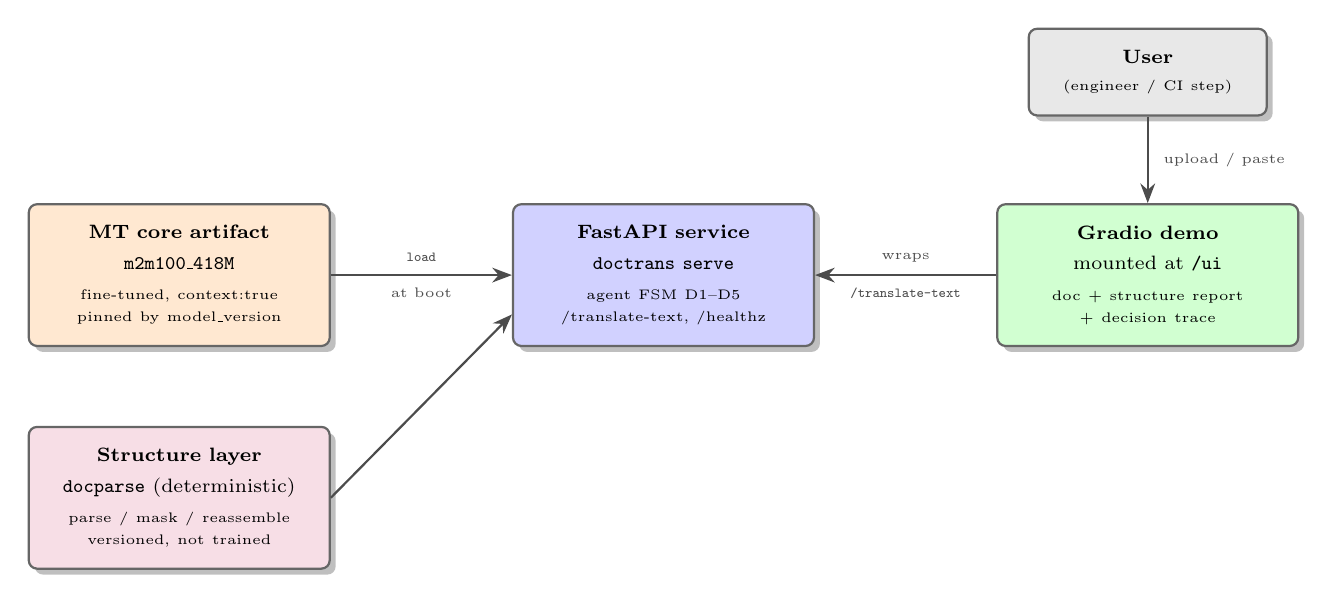
\begin{tikzpicture}[
  node distance=1.0cm and 2.3cm,
  box/.style={rectangle, draw=black!60, rounded corners=3pt, thick,
             text width=3.4cm, minimum height=1.8cm, align=center,
             inner sep=6pt, font=\scriptsize, drop shadow},
  modelbox/.style={box, fill=orange!18},
  structbox/.style={box, fill=purple!13},
  apibox/.style={box, fill=blue!18},
  uibox/.style={box, fill=green!18},
  userbox/.style={box, fill=gray!18, text width=2.6cm, minimum height=1.1cm},
  arrow/.style={-{Stealth[length=2.5mm]}, thick, color=black!70}
]

\node[modelbox] (mt) {%
  \textbf{MT core artifact}\\[3pt]
  \texttt{m2m100\_418M}\\[3pt]
  {\tiny fine-tuned, context:true}\\
  {\tiny pinned by model\_version}
};
\node[structbox, below=1.0cm of mt] (struct) {%
  \textbf{Structure layer}\\[3pt]
  \texttt{docparse} (deterministic)\\[3pt]
  {\tiny parse / mask / reassemble}\\
  {\tiny versioned, not trained}
};
\node[apibox, right=of mt] (api) {%
  \textbf{FastAPI service}\\[3pt]
  \texttt{doctrans serve}\\[3pt]
  {\tiny agent FSM D1--D5}\\
  {\tiny /translate-text, /healthz}
};
\node[uibox, right=of api] (ui) {%
  \textbf{Gradio demo}\\[3pt]
  mounted at \texttt{/ui}\\[3pt]
  {\tiny doc + structure report}\\
  {\tiny + decision trace}
};
\node[userbox, above=1.1cm of ui] (user) {%
  \textbf{User}\\[2pt]
  {\tiny (engineer / CI step)}
};

\draw[arrow] (mt.east) -- node[above=1pt, font=\tiny] {\texttt{load}} node[below=1pt, font=\tiny] {at boot} (api.west);
\draw[arrow] (struct.east) -- ([yshift=-5mm]api.west);
\draw[arrow] (ui.west) -- node[above=1pt, font=\tiny] {wraps} node[below=1pt, font=\tiny] {\texttt{/translate-text}} (api.east);
\draw[arrow] (user) -- node[right=2pt, font=\tiny] {upload / paste} (ui);

\end{tikzpicture}%
}
\caption{Serving architecture. The deterministic structure layer and the pinned MT core artifact are both loaded by the FastAPI service; the Gradio demo wraps \texttt{/translate-text}. The model never sees structure and the structure layer never sees the model -- two artifacts, two lifecycles.}
\label{fig:arch}
\end{figure}

\subsection{FastAPI Endpoints}

\begin{table}[H]
\centering
\caption{FastAPI surface}
\small
\begin{tabularx}{\linewidth}{@{} l l L @{}}
\toprule
\textbf{Method} & \textbf{Path} & \textbf{Description} \\
\midrule
\texttt{POST} & \texttt{/translate-text} & JSON in (\texttt{\{text, fmt\}}), JSON out: \texttt{\{translated, fmt, structure\_report, decision\_trace\}}; \texttt{fmt} defaults to \texttt{auto} (D1 detection). \\
\texttt{POST} & \texttt{/translate-document} & \texttt{multipart/form-data} file upload; byte-stable in the uploaded format. \textbf{Registered only when \texttt{python-multipart} is present} (multipart-gated). \\
\texttt{GET} & \texttt{/healthz} & Liveness probe for Docker/Spaces; no model load. \\
\texttt{GET} & \texttt{/version} & Returns \texttt{\{package, model\_version, context\}}. \\
\bottomrule
\end{tabularx}
\end{table}

\textbf{Multipart gating (a load-bearing P05/P13 lesson):} \texttt{UploadFile}/\texttt{File()} routes hard-require \texttt{python-multipart}; without it FastAPI raises at route registration. The \texttt{/translate-document} route is therefore gated so \texttt{/translate-text}, \texttt{/healthz}, and \texttt{/version} still work if multipart is absent -- the core service never fails to boot over an optional dependency.

\subsection{Gradio Demo}

A single-page Gradio app wraps \texttt{/translate-text}: paste a Markdown/HTML/JSON/plain document, pick a format (or \texttt{auto}), and see the rendered translated document, the structure-preservation report, and the per-segment D1--D5 decision trace side by side. It is mounted under FastAPI (\texttt{gr.mount\_gradio\_app(app, demo, path="/ui")}) so one process serves API + UI.

\subsection{Offline Degradation and Versioning}

Every heavy import is lazy, so the package boots and serves with the minimal stack. When torch/transformers are unavailable, parsers fall back native $\rightarrow$ regex $\rightarrow$ plain and the MT core falls back to the offline dictionary translator over the seed; structure preservation is unaffected (deterministic), so round-trip identity, masking, and SPS still hold offline. \texttt{model\_version} is pinned at startup and surfaced via \texttt{/version}; the continual-learning loop only advances it after the chrF non-regression gate passes.

% ============================================================
\section{Agentic AI Component}
% ============================================================

\subsection{Agent Architecture}

The \texttt{doctrans} agent is a \textbf{deterministic finite-state machine (FSM)}, not an LLM controller. Given the same document and model it always takes the same path and emits the same audit trace. It orchestrates the deterministic localization spine and calls the only learned component -- the MT model -- through an opaque interface, so the agent never reasons about structure and the model never sees it.

Every action is a \textbf{tool} behind one signature: it receives a typed input, returns a typed output plus a status (\texttt{ok} / \texttt{flag} / \texttt{abort}), and appends a \texttt{ToolStep} to a shared \texttt{ToolTrace} (tool name, inputs digest, output digest, the gate decision, and any threshold checked). The \texttt{ToolTrace} is the audit log returned in every API response, so a reviewer can replay exactly why a document passed, was flagged, or fell back to source.

\begin{figure}[H]
\centering
\resizebox{\linewidth}{!}{%
\begin{tikzpicture}[
  node distance=0.32cm,
  step/.style={rectangle, draw=black!60, rounded corners=2pt, thick,
              text width=13.5cm, inner sep=5pt, minimum height=0.7cm,
              align=center, font=\footnotesize},
  d1/.style={step, fill=gray!15},
  d2/.style={step, fill=blue!15},
  d3/.style={step, fill=orange!15},
  d4/.style={step, fill=red!12},
  d5/.style={step, fill=green!15},
  arrow/.style={-{Stealth[length=2mm]}, thick}
]

\node[d1] (a1) {\textbf{D1 -- Format detect + parse} (\textit{tool}): ext $\rightarrow$ MIME $\rightarrow$ content sniff; \textbf{round-trip identity} \texttt{reserialize(parse(x))==x}};
\node[d2, below=of a1] (a2) {\textbf{D2 -- Segment + mask} (\textit{decision}): skip if letter-ratio $<$ 0.30; mask code/URLs/placeholders as reversible \texttt{[[PHn]]} sentinels};
\node[d3, below=of a2] (a3) {\textbf{D3 -- Translate with $k$ context} (\textit{multi-step reasoning + tool}): concat-$k$ MT; reject empty / length-ratio outside $[0.4, 3.0]$};
\node[d4, below=of a3] (a4) {\textbf{D4 -- Verify gate} (\textit{decision}): \textbf{placeholder-retention HARD} (each \texttt{[[PHn]]} back exactly once) + back-translation chrF $\geq 0.30$ (soft)};
\node[d5, below=of a4] (a5) {\textbf{D5 -- Reassemble + structure-validate} (\textit{tool}): unmask 1:1 $\rightarrow$ slot leaves into untouched skeleton $\rightarrow$ structure-signature match + re-parse};

\foreach \a/\b in {a1/a2, a2/a3, a3/a4, a4/a5}
  \draw[arrow] (\a) -- (\b);

% feedback / fail arrows
\draw[arrow, dashed, color=red!70] (a4.west) to[bend left=55] node[left, font=\tiny] {fail: re-translate $\leq N{=}2$} (a3.west);
\draw[arrow, dashed, color=red!70] (a5.east) to[bend right=55] node[right, font=\tiny] {fail: repair $\leq M{=}1$} (a5.east);

\end{tikzpicture}%
}
\caption{The deterministic agent FSM with five decision gates. The path is \texttt{IN $\rightarrow$ D1 $\rightarrow$ D2 $\rightarrow$ D3 $\rightarrow$ D4 (pass) $\rightarrow$ D5 (pass) $\rightarrow$ OUT}. D4 failure loops to D3 (budget $N=2$); D5 repair budget $M=1$. Budgets are finite by design, so the FSM never loops and termination is guaranteed.}
\label{fig:agent}
\end{figure}

\subsection{The Five Decision Gates (D1--D5)}

\begin{table}[H]
\centering
\caption{The five decision gates, their hard checks, and fail actions}
\small
\begin{tabularx}{\linewidth}{@{} l L L @{}}
\toprule
\textbf{Gate} & \textbf{Decision \& hard check} & \textbf{On failure} \\
\midrule
\textbf{D1} Format detect + parse & Route by format; \textbf{round-trip identity}: skeleton + segments re-join byte-for-byte & Degrade native $\rightarrow$ regex $\rightarrow$ plain; hard parse failure $\rightarrow$ flag/abort \\
\textbf{D2} Segment + mask & Skip non-text by \textbf{letter-ratio $<$ 0.30}; masks reversible \& balanced (each \texttt{[[PHi]]} $\leftrightarrow$ one literal, contiguous indices) & Skip segment as literal; unbalanced masks $\rightarrow$ flag, pass through verbatim \\
\textbf{D3} Translate ($k$ context) & Translate with concat-$k$; reject empty output or \textbf{length-ratio outside $[0.4, 3.0]$} & Re-translate, budget $N=2$ (shrink $k$, then mask harder); then flag \\
\textbf{D4} Verify gate & \textbf{(1) placeholder-retention HARD} (each \texttt{[[PHi]]} back exactly once); \textbf{(2) back-translation chrF $\geq 0.30$} (soft) & Retention fail $\rightarrow$ flag/abort; loop to D3 $\leq N$; then emit best-of + flag \\
\textbf{D5} Reassemble + validate & Unmask 1:1 $\rightarrow$ slot leaves into skeleton; \textbf{structure-signature match} + zero residual sentinels + re-parses cleanly & Repair, budget $M=1$; else flag document, fail-soft keep source + diff report \\
\bottomrule
\end{tabularx}
\end{table}

\textbf{D4 placeholder-retention is the one non-negotiable HARD gate}: a translation that drops or duplicates a sentinel can never ship, because restoring masks would corrupt the document. An optional \texttt{anthropic} LLM ``brain'' (\textbf{OFF by default}) is a strict-superset advisory layer: it may write a terminology-consistency note but \textbf{never} rewrites a translation, changes structure, or touches placeholders, and anything it influences re-enters the same gates.

\subsection{Example Trace}

\begin{lstlisting}
# Example -- a Markdown document with a heading, a placeholder, and a link
Input  (sample.md):
  "# Welcome, {user}\nSee the [docs](https://example.com/help)."

  D1 Format detect + parse:
     fmt=markdown; round-trip identity OK (reserialize(parse(x))==x)
  D2 Segment + mask:
     seg0 "# Welcome, {user}"  -> mask -> "Welcome, [[PH0]]"  (heading hash skeleton)
     seg1 "See the [docs](...)" -> mask -> "See the [[PH1]]docs[[PH2]]."
        mask_map = {PH0:"{user}", PH1:"[", PH2:"](https://example.com/help)"}
  D3 Translate (k context):
     seg0 -> "Bienvenue, [[PH0]]"
     seg1 -> "Consultez la [[PH1]]docs[[PH2]]."
     length-ratio in [0.4, 3.0] -> OK
  D4 Verify gate:
     placeholder-retention: {PH0,PH1,PH2} in == out, each once -> HARD PASS
     back-translation chrF = 0.71 (>= 0.30) -> PASS
  D5 Reassemble + structure-validate:
     unmask 1:1 -> "# Bienvenue, {user}\nConsultez la [docs](https://example.com/help)."
     structure-signature match (1 heading, 1 link) + re-parses -> PASS
Output (sample.fr.md):  structure byte-stable, placeholders intact, prose in French
  action=OK, SPS=1.0, placeholder_retention=1.0, model_used=m2m100:context
\end{lstlisting}

% ============================================================
\section{Continual Learning \& Monitoring}
% ============================================================

\subsection{Two Artifacts, Two Lifecycles}

The guiding split: \textbf{the MT core is trainable and re-fine-tuned on a loop; the structure layer is deterministic code that is versioned, never trained.} Structure reproducibility is a code-level guarantee independent of model weights.

\subsection{The Re-Fine-Tune Loop (MT core only)}

\begin{enumerate}\setlength\itemsep{0.15em}
  \item \textbf{Collect}: gather in-domain documents plus human references -- ideally the segments the agent flagged for review (D3/D4/D5), since those are exactly where the model is weakest. Re-running the spine yields aligned \texttt{(source segment, gold target)} pairs already shorn of structure.
  \item \textbf{Build context}: re-apply concat-$k$ ($k=2$, source-side, left-truncated) so new data trains document-level behavior; new checkpoints keep \texttt{context:true}.
  \item \textbf{Train}: HF \texttt{Seq2SeqTrainer}, resume-safe, re-fine-tuning the existing checkpoint (not from scratch).
  \item \textbf{Gate}: promote only if the chrF non-regression gate passes.
  \item \textbf{Promote}: passing checkpoints become a new \texttt{model\_version}; the structure-layer version is unchanged.
\end{enumerate}

\begin{table}[H]
\centering
\caption{The chrF non-regression promotion gate (on a frozen held-out set)}
\small
\begin{tabularx}{\linewidth}{@{} l L l @{}}
\toprule
\textbf{Check} & \textbf{Rule} & \textbf{On fail} \\
\midrule
Headline chrF & \texttt{chrF\_new $\geq$ chrF\_prod $-\,\epsilon$} ($\epsilon\approx0.5$) & reject \\
Document chrF (d-chrF) & no regression on doc-level set & reject \\
SPS & $\geq$ current (deterministic; should hold) & investigate structure layer \\
Sanity floors & beats identity ($\sim$21) and dictionary ($\sim$82 offline) & reject \\
\bottomrule
\end{tabularx}
\end{table}

\subsection{Monitoring}

Production logs are \textbf{metadata-only} (no document bodies). Three live signals are rolled up:

\begin{table}[H]
\centering
\caption{Operational monitor-log signals}
\small
\begin{tabularx}{\linewidth}{@{} l L l @{}}
\toprule
\textbf{Signal} & \textbf{What it catches} & \textbf{Drift} \\
\midrule
\textbf{needs-review rate} & rising D3/D4/D5 flags $=$ model losing the domain & up $=$ bad \\
\textbf{mean SPS} & structure breakage (struct $\times$ markup $\times$ PHR) & down $=$ bad \\
\textbf{latency} & context length / retry-budget creep & up $=$ watch \\
\bottomrule
\end{tabularx}
\end{table}

Rising needs-review \emph{and} falling SPS together is the canonical drift signal and a trigger to start a new collect step. \textbf{Monitoring} (``is it healthy?'') and \textbf{observability} (the per-request \texttt{ToolTrace} that answers ``why did \emph{this} document fail?'') are both provided; because the structure layer is deterministic, any structure failure is fully reproducible from its trace and fixed in code under a new structure-layer version, never by retraining. \textbf{Alarm fatigue} is managed by keeping HARD gates strict and the SOFT gates (back-translation chrF $\geq 0.30$, length-ratio $[0.4, 3.0]$) calibrated so the needs-review rate stays actionable.

% ============================================================
\section{Data Privacy \& Model Robustness}
% ============================================================

\subsection{Privacy}

Documents may carry confidential prose, internal URLs, customer placeholders, or embedded metadata, so \texttt{doctrans} minimizes exposure:
\begin{itemize}
  \item \textbf{Local-first, offline-capable}: the package runs with only \texttt{numpy/scikit-learn/pyyaml/pydantic}; with the offline seed the full pipeline runs with \textbf{no network and no torch}, so documents never leave the machine.
  \item \textbf{Local path I/O}: inputs/outputs are scoped by \texttt{DOCTRANS\_DATA\_DIR} / \texttt{\_ARTIFACTS\_DIR} / \texttt{\_RUN\_DIR}; \texttt{HF\_HOME} scopes any model cache.
  \item \textbf{Metadata-only logging}: the FastAPI service logs format, segment count, decision trace, SPS, and latency -- \textbf{never} document content. Decision traces reference segments by index/sentinel, not raw payload.
  \item \textbf{Optional LLM brain is OFF by default}: leaving it off keeps all text on-device; even when enabled it writes only a terminology note and never sees structure or placeholders.
\end{itemize}

\subsection{Robustness}

\begin{itemize}\setlength\itemsep{0.15em}
  \item \textbf{Structure-corruption prevention}: three deterministic gates -- round-trip identity (D1), a byte-stable skeleton the model never sees, and structure-validate (D5, repair budget $M=1$).
  \item \textbf{Placeholder / markup loss}: non-translatable spans are masked as reversible, cp1252-safe \texttt{[[PHn]]} sentinels with a HARD retention gate (D4), a re-translate budget $N=2$ on length-ratio/emptiness violations (D3), and a soft back-translation chrF $\geq 0.30$ check.
  \item \textbf{Graceful degradation}: parser ladder native $\rightarrow$ regex $\rightarrow$ plain; MT fallback ladder trained m2m100 $\rightarrow$ zero-shot $\rightarrow$ dictionary $\rightarrow$ identity, so a translation always returns something inspectable.
  \item \textbf{Abstention is first-class}: any gate failure raises the needs-review flag instead of forcing output; unrecoverable failure fails soft and keeps the source.
\end{itemize}

% ============================================================
\section{Project Management}
% ============================================================

This project was completed \textit{individually} (Le Dinh Minh Quan, 23127460). The build follows the localization spine bottom-up so each layer is testable before the next depends on it.

\begin{table}[H]
\centering
\caption{Build order / project timeline (dependency-ordered)}
\small
\begin{tabularx}{\linewidth}{@{} l l L @{}}
\toprule
\textbf{Stage} & \textbf{Days} & \textbf{Exit criterion} \\
\midrule
0 Foundations & 1--2 & config + logging + registry + offline seed run with core deps only \\
1 Structure layer & 3--5 & \textbf{D1 round-trip identity} (re-join $==$ source byte-for-byte) on seed \\
2 MT core + context & 6--8 & dictionary MT beats identity floor; concat-$k$ builder ($k$=2, \texttt{<BRK>}) \\
3 Training + eval & 9--12 & \texttt{doctrans evaluate} emits versioned JSON metrics + 2$\times$2 ablation \\
4 Agent & 13--14 & end-to-end translate with full D1--D5 decision trace \\
5 API / UI / CLI & 15--16 & endpoints return doc + structure report + trace; Gradio at \texttt{/ui} \\
6 Reports / ops & 17--20 & non-regression gate green; report + slides reproduce; grading PASS \\
\bottomrule
\end{tabularx}
\end{table}

\textbf{Scaling reflection}: in a team setting the stages would parallelize (structure layer / MT training / agent+API / monitoring+report) once the \texttt{Segment}/\texttt{mask\_map} interface and the versioned-JSON metric contract are fixed. CI runs CPU-only on the offline seed, so correctness is verifiable without a GPU.

% ============================================================
\section{Ethics \& Responsible AI}
% ============================================================

\subsection{Stance: a Localization Aid, Not an Autonomous Translator}

\texttt{doctrans} \emph{assists} a human localizer; it does \textbf{not} ship final translations unattended. The deterministic agent enforces this: any output that breaks structure or falls below a confidence gate is \textbf{flagged for human review} and never presented as final. When the agent cannot produce a verified document it \textbf{fails soft} -- it keeps the \emph{source} document intact rather than emit a corrupted translation. Silence-with-source beats a confident wrong answer.

\subsection{Who Benefits, Who Could Be Harmed}

Localization engineers, documentation teams, and i18n owners benefit from faster, structure-safe translation. Potential harms arise from \textbf{mistranslation} in legal/medical/financial documents (out of scope for unreviewed use; flagged by D4 soft gates) and from \textbf{uneven quality} across domains and discourse (addressed by concat-$k$ context and reported per-domain, not as a single number).

\subsection{Primary Risks and Mitigations}

\begin{table}[H]
\centering
\caption{Risks and mitigations}
\small
\begin{tabularx}{\linewidth}{@{} L L @{}}
\toprule
\textbf{Risk} & \textbf{Mitigation in \texttt{doctrans}} \\
\midrule
Mistranslation harm & Output advisory; D4 back-translation chrF + length-ratio bounds flag suspect segments; domain-critical content out of scope for unreviewed use \\
Structure / placeholder corruption & HARD gates: D1 round-trip identity, D4 placeholder-retention, D5 structure-signature match + re-parse; repair then fail-soft to source \\
Bias across languages/domains & concat-$k$ context targets discourse consistency; honest caveat published; reported per-domain \\
License misuse & Per-asset license flags; clean path m2m100 (MIT) + offline seed; non-commercial assets flagged, never silently shipped \\
Over-trust / automation bias & UI/report always surface the decision trace + structure report; flagged segments visibly marked \\
Privacy & Metadata-only request logging; document bodies never retained; offline-capable \\
\bottomrule
\end{tabularx}
\end{table}

\subsection{Human-in-the-Loop and Accountability}

Each of the agent's five decisions emits a \texttt{ToolTrace}; a human reviewer is the final authority on any flagged document. Numbers in the docs are illustrative of the verified offline path -- live figures are reproduced by running \texttt{doctrans evaluate}. The structure layer is deterministic, versioned code: auditable and not subject to model drift. \textbf{Bottom line:} preserve the document, surface uncertainty, keep a human in charge, and respect data/model licenses.

\end{document}
